\documentclass[border=2mm]{standalone}
\usepackage[utf8]{inputenc}
\usepackage{tikz}
\usetikzlibrary{shapes,arrows,calc}

\begin{document}
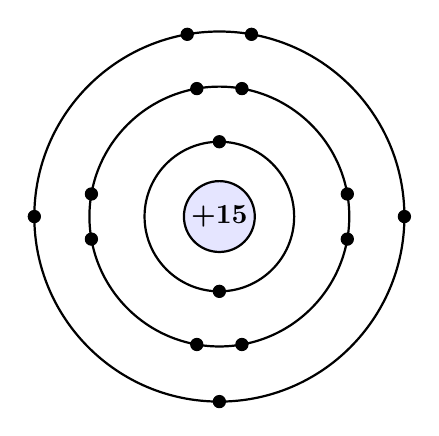
\begin{tikzpicture}[>=latex, line cap=round]
    % Central nucleus
    \draw[thick, fill=blue!10] (0,0) circle (0.45cm);
    \node at (0,0) {\textbf{+15}};

    % Shell 1 (K)
    \draw[thick] (0,0) circle (0.95cm);
    \filldraw[fill=black] (0, 0.95) circle (2.2pt);
    \filldraw[fill=black] (0, -0.95) circle (2.2pt);

    % Shell 2 (L)
    \draw[thick] (0,0) circle (1.65cm);
    % 4 pairs
    \filldraw[fill=black] ({1.65*cos(80)}, {1.65*sin(80)}) circle (2.2pt);
    \filldraw[fill=black] ({1.65*cos(100)}, {1.65*sin(100)}) circle (2.2pt);
    \filldraw[fill=black] ({1.65*cos(260)}, {1.65*sin(260)}) circle (2.2pt);
    \filldraw[fill=black] ({1.65*cos(280)}, {1.65*sin(280)}) circle (2.2pt);
    \filldraw[fill=black] ({1.65*cos(170)}, {1.65*sin(170)}) circle (2.2pt);
    \filldraw[fill=black] ({1.65*cos(190)}, {1.65*sin(190)}) circle (2.2pt);
    \filldraw[fill=black] ({1.65*cos(-10)}, {1.65*sin(-10)}) circle (2.2pt);
    \filldraw[fill=black] ({1.65*cos(10)}, {1.65*sin(10)}) circle (2.2pt);

    % Shell 3 (M)
    \draw[thick] (0,0) circle (2.35cm);
    % 5 electrons: 1 pair at top, 1 at right, 1 at bottom, 1 at left
    \filldraw[fill=black] ({2.35*cos(80)}, {2.35*sin(80)}) circle (2.2pt);
    \filldraw[fill=black] ({2.35*cos(100)}, {2.35*sin(100)}) circle (2.2pt);
    \filldraw[fill=black] ({2.35*cos(0)}, {2.35*sin(0)}) circle (2.2pt);
    \filldraw[fill=black] ({2.35*cos(270)}, {2.35*sin(270)}) circle (2.2pt);
    \filldraw[fill=black] ({2.35*cos(180)}, {2.35*sin(180)}) circle (2.2pt);
\end{tikzpicture}
\end{document}
